% This template has been tested with LLNCS DOCUMENT CLASS -- version 2.20 (24-JUN-2015)

%"runningheads" enables:
%  - page number on page 2 onwards
%  - title/authors on even/odd pages
%This is good for other readers to enable proper archiving among other papers and pointing to content.
%Even if the title page states the title, when printed and stored in a folder, when blindly opening the folder, one could hit not the title page, but an arbitrary page. Therefore, it is good to have title printed on the pages, too.
\documentclass[runningheads,a4paper]{llncs}

%cmap has to be loaded before any font package (such as cfr-lm)
\usepackage{cmap}
\usepackage[T1]{fontenc}

\usepackage{graphicx}

%Even though `american`, `english` and `USenglish` are synonyms for babel package (according to https://tex.stackexchange.com/questions/12775/babel-english-american-usenglish), the llncs document class is prepared to avoid the overriding of certain names (such as "Abstract." -> "Abstract" or "Fig." -> "Figure") when using `english`, but not when using the other 2.
%english has to go last to set it as default language
\usepackage[ngerman,english]{babel}
%Hint by http://tex.stackexchange.com/a/321066/9075 -> enable "= as dashes
\addto\extrasenglish{\languageshorthands{ngerman}\useshorthands{"}}

%better font, similar to the default springer font
%cfr-lm is preferred over lmodern. Reasoning at http://tex.stackexchange.com/a/247543/9075
\usepackage[%
rm={oldstyle=false,proportional=true},%
sf={oldstyle=false,proportional=true},%
tt={oldstyle=false,proportional=true,variable=true},%
qt=false%
]{cfr-lm}
%
%if more space is needed, exchange cfr-lm by mathptmx
%\usepackage{mathptmx}

%for demonstration purposes only
\usepackage[math]{blindtext}

%Sorts the citations in the brackets
%It also allows \cite{refa, refb}. Otherwise, the document does not compile.
%  Error message: "White space in argument"
\usepackage{cite}


%% If you need packages for other papers,
%% START COPYING HERE
%% COPY ALSO cmap and fontenc from lines 10 to 12

%extended enumerate, such as \begin{compactenum}
\usepackage{paralist}

%put figures inside a text
%\usepackage{picins}
%use
%\piccaptioninside
%\piccaption{...}
%\parpic[r]{\includegraphics ...}
%Text...

%for easy quotations: \enquote{text}
\usepackage{csquotes}

%enable margin kerning
\usepackage{microtype}

%tweak \url{...}
\usepackage{url}
%\urlstyle{same}
%improve wrapping of URLs - hint by http://tex.stackexchange.com/a/10419/9075
\makeatletter
\g@addto@macro{\UrlBreaks}{\UrlOrds}
\makeatother
%nicer // - solution by http://tex.stackexchange.com/a/98470/9075
%DO NOT ACTIVATE -> prevents line breaks
%\makeatletter
%\def\Url@twoslashes{\mathchar`\/\@ifnextchar/{\kern-.2em}{}}
%\g@addto@macro\UrlSpecials{\do\/{\Url@twoslashes}}
%\makeatother

%diagonal lines in a table - http://tex.stackexchange.com/questions/17745/diagonal-lines-in-table-cell
%slashbox is not available in texlive (due to licensing) and also gives bad results. This, we use diagbox
%\usepackage{diagbox}

%required for pdfcomment later
\usepackage{xcolor}


%enable nice comments
%this also loads hyperref
\usepackage{pdfcomment}
%enable hyperref without colors and without bookmarks
\hypersetup{hidelinks,
   colorlinks=true,
   allcolors=black,
   pdfstartview=Fit,
   breaklinks=true}
%enables correct jumping to figures when referencing
\usepackage[all]{hypcap}

\newcommand{\commentontext}[2]{\colorbox{yellow!60}{#1}\pdfcomment[color={0.234 0.867 0.211},hoffset=-6pt,voffset=10pt,opacity=0.5]{#2}}
\newcommand{\commentatside}[1]{\pdfcomment[color={0.045 0.278 0.643},icon=Note]{#1}}

%compatibality with packages todo, easy-todo, todonotes
\newcommand{\todo}[1]{\commentatside{#1}}
%compatiblity with package fixmetodonotes
\newcommand{\TODO}[1]{\commentatside{#1}}

%enable \cref{...} and \Cref{...} instead of \ref: Type of reference included in the link
\usepackage[capitalise,nameinlink]{cleveref}
%Nice formats for \cref
\crefname{section}{Sect.}{Sect.}
\Crefname{section}{Section}{Sections}

\usepackage{xspace}
%\newcommand{\eg}{e.\,g.\xspace}
%\newcommand{\ie}{i.\,e.\xspace}
\newcommand{\eg}{e.\,g.,\ }
\newcommand{\ie}{i.\,e.,\ }

%introduce \powerset - hint by http://matheplanet.com/matheplanet/nuke/html/viewtopic.php?topic=136492&post_id=997377
\DeclareFontFamily{U}{MnSymbolC}{}
\DeclareSymbolFont{MnSyC}{U}{MnSymbolC}{m}{n}
\DeclareFontShape{U}{MnSymbolC}{m}{n}{
    <-6>  MnSymbolC5
   <6-7>  MnSymbolC6
   <7-8>  MnSymbolC7
   <8-9>  MnSymbolC8
   <9-10> MnSymbolC9
  <10-12> MnSymbolC10
  <12->   MnSymbolC12%
}{}
\DeclareMathSymbol{\powerset}{\mathord}{MnSyC}{180}

% correct bad hyphenation here
\hyphenation{op-tical net-works semi-conduc-tor}
%Make plots
\usepackage{pgfplotstable}
\usepackage{pgfplots}

\pgfplotsset{compat=1.15}

\usepackage{graphicx}
\usepackage{subcaption}
\graphicspath{ {images/} }
%% END COPYING HERE


\begin{document}

\title{Blinking Extraction in Eye gaze System for Stereoscopy Movies}
%If Title is too long, use \titlerunning
%\titlerunning{Short Title}

%Single insitute
\author{Filip Rynkiewicz \and Piotr Napieralski}
%If there are too many authors, use \authorrunning
%\authorrunning{First Author et al.}
\institute{Institute of Information Technology, Lodz University of Technology}

%Multiple insitutes
%Currently disabled
%
\iffalse
%Multiple institutes are typeset as follows:
\author{Firstname Lastname\inst{1} \and Firstname Lastname\inst{2} }
%If there are too many authors, use \authorrunning
%\authorrunning{First Author et al.}

\institute{
Insitute 1\\
\email{...}\and
Insitute 2\\
\email{...}
}
\fi


\maketitle
\iffalse
\begin{abstract}
Abstract goes here
\end{abstract}
\fi
\begin{keywords}
data science algorithms, stereoscopy, blinking extraction, Eye-gaze systems
\end{keywords}

%%%%%%%%%%%%%%%%%%%%%%%%%%%%%%%%%%%%%%%%%%%%%%%%%%%%%%%%%%%%%%%%%%%%%%%%%%%%%%%
\section{Introduction}\label{sec:intro}
%%%%%%%%%%%%%%%%%%%%%%%%%%%%%%%%%%%%%%%%%%%%%%%%%%%%%%%%%%%%%%%%%%%%%%%%%%%%%%%
Gaze motion research has started in 1879 when French ophthalmologist Louis Emile Javal came to conclusion that observer does not sweep smoothly along the text with his eyes, but with a series of stops and quick saccades\cite{Winery}.  Since his first observation, the eye-tracking devices was developed. Firstly, those devices were very simple, readers had to wear a type of contact lens with a small opening for the pupil. The lens was attached to a pointer which changed its position following the movements of the eye. The significance of those studies has led to a growth of new, more complicated devices that can automatically measure gaze point. The most common devices are from Tobii and EyeTribe company.


\section{Tobii X2}
The Tobii X2 is a standalone eyetracker that can be used in various setups  by attaching it to monitors, laptops or for performing eye tracking on physical objects. It have sampling rate 60Hz and system latency under 35ms and it is aimed at determining precisely where the participants are looking, the gaze point, timing, duration of fixations and eye movements such as saccades, for example. This device using Tobii EyeCore\textsuperscript{\tiny\textregistered} algorithm.
\section{EyeTribe}
Second device is also capable of sampling data in 30Hz and 60Hz with less than 20ms latency at 60Hz. This equipment have a way worse precision and has more trouble compensating for users that move their head when being tracked. 

\section{Blink extraction}
Tracking of eye gaze and movement are based on searching the pupil center, pupil ellipse, the shape of eye etc. Blinking is most often an involuntary act of shutting and opening the eyelid. When it occurs the eye is automatically closed, so the the position of it will be lost. Thats why filtering noise caused by blinking is an important task. 
\par As it can be seen at \figurename\ref{fig:data} gaze point from movie can be visualized as set of 2d points or degrees. But when blinking occurs the position of gaze are automatically set to $(0,0)$ point. In \cite{4274377} the way to compensate was proposed, simple feedback loop with a delay factor \figurename\ref{fig:3}

\begin{figure}
\centering

\begin{tikzpicture}[domain=0:3,scale=0.8]
\begin{axis}[
enlargelimits=true,
xlabel=x coordinates of gaze point,
ylabel=y coordinates of gaze point
]
\addplot+[
only marks,
scatter,
mark=halfcircle*,
mark size=3.0pt,
]
table[x=pos_x_1m_normalized,y=pos_y_1m_normalized]
{data.dat};
\end{axis}
\end{tikzpicture}
\caption{Gaze point gathered from movie.} \label{fig:data}

		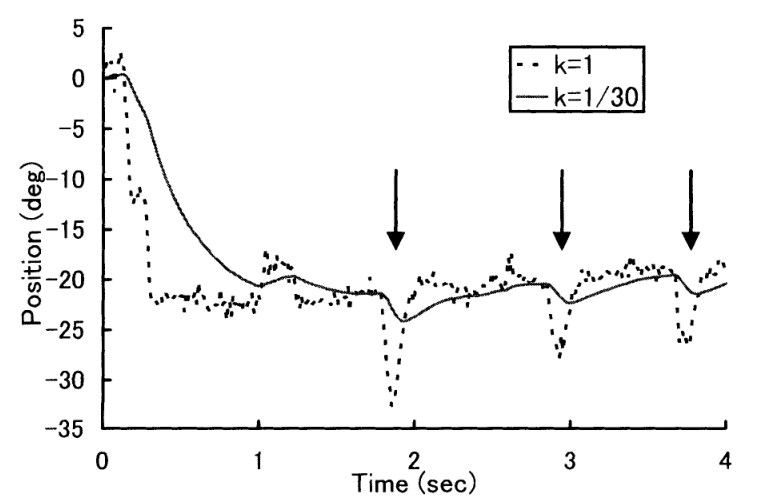
\includegraphics[height=5cm ,width=7cm]{blinkReduction.png}
	\caption{The proposed signal processing procedure reduced the blinking
		effect.\cite{4274377}}\label{fig:3}


\end{figure}


%%%%%%%%%%%%%%%%%%%%%%%%%%%%%%%%%%%%%%%%%%%%%%%%%%%%%%%%%%%%%%%%%%%%%%%%%%%%%%%
\bibliographystyle{splncs03}
\bibliography{paper}

All links were last followed on \today
%%%%%%%%%%%%%%%%%%%%%%%%%%%%%%%%%%%%%%%%%%%%%%%%%%%%%%%%%%%%%%%%%%%%%%%%%%%%%%%

\end{document}
